\section{본 론}

사용자 $i$의 프로필 이미지를 $x_i$라 정의한다. 커플 쌍 $(x_f, x_m)$에 대해, 두 사용자의 임베딩 $e_f$, $e_m$이 임베딩 공간에서 가깝도록 학습하며, 비커플 쌍은 멀어지도록 대조 학습을 수행한다. 실제 데이팅 앱에서 상호 좋아요를 통해 매칭된 커플 495쌍의 프로필 이미지를 수집하였으며, Train 346쌍(70\%), Validation 74쌍(15\%), Test 75쌍(15\%)으로 분할하였다.

그림 \ref{fig:architecture}는 제안 모델의 전체 아키텍처를 나타낸다. 대규모 데이터로 사전 학습된 Qwen3-VL-2B\cite{qwen2023}를 백본으로 사용한다. Qwen3-VL은 이미지와 텍스트를 함께 이해하는 비전-언어 모델로, 다양한 시각적 태스크에서 뛰어난 일반화 성능을 보인다. 소규모 도메인 데이터에서의 과적합을 방지하기 위해, 백본 네트워크의 약 20억 개 파라미터는 모두 동결한다.

\begin{figure}[h]
\centering
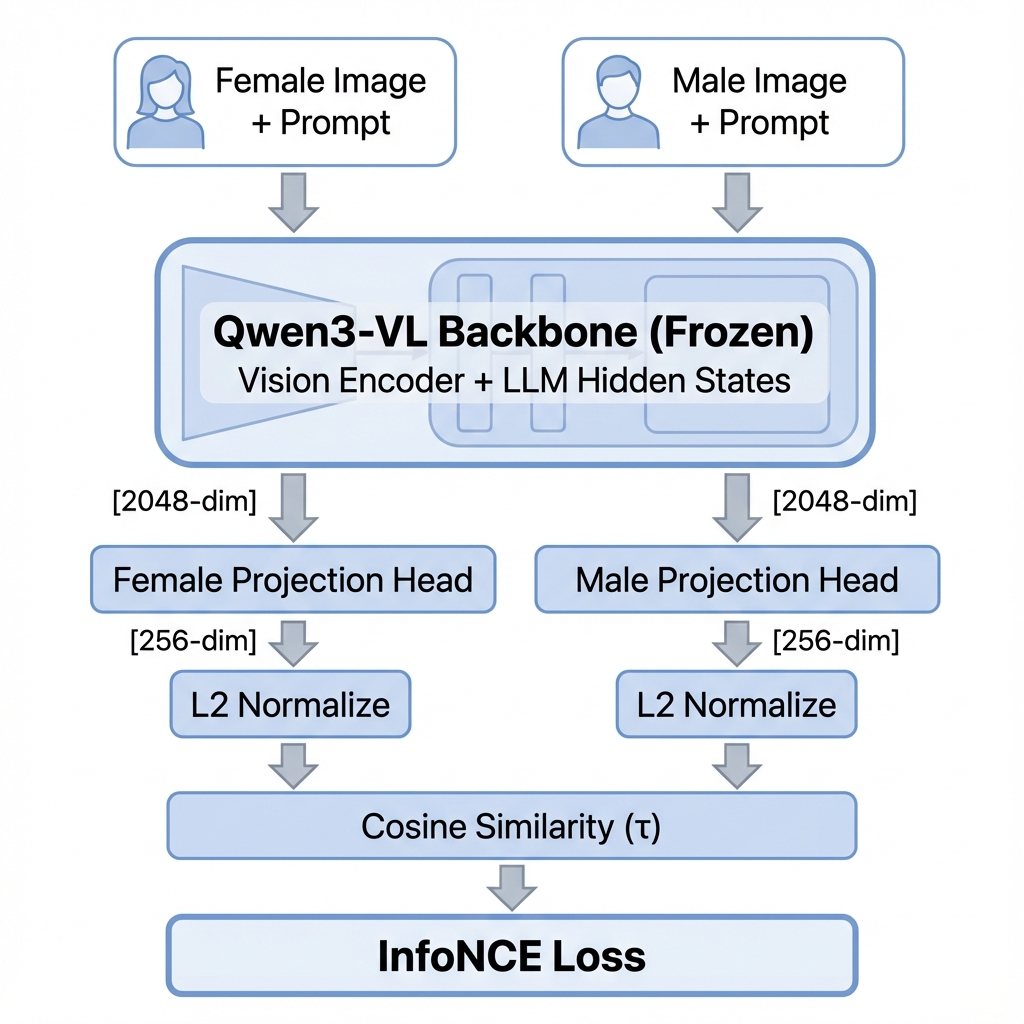
\includegraphics[width=0.9\columnwidth]{figures/model_architecture.png}
\caption{제안 모델의 전체 아키텍처}
\label{fig:architecture}
\end{figure}

VLM의 멀티모달 이해 능력을 활용하기 위해, 이미지와 함께 구조화된 텍스트 프롬프트를 입력으로 사용한다. 텍스트 프롬프트는 성별별 시스템 프롬프트와 이미지 분석 요청으로 구성되며, VLM이 매칭 호환성 관련 시각적 특징을 추출하도록 유도한다.

백본을 통과한 고차원 특징 벡터 $h_i$는 식 (1)과 같다.

\begin{equation}
h_i = f_\theta(x_i) \in \mathbb{R}^{2048}
\end{equation}

매칭 호환성 학습에 특화된 저차원 임베딩을 얻기 위해, 학습 가능한 프로젝션 헤드 $g_\phi$를 추가한다. 프로젝션 헤드는 2개의 선형 계층과 BatchNorm, ReLU 활성 함수로 구성된다.

\begin{equation}
z_i = g_\phi(h_i) = W_2 \cdot \text{ReLU}(\text{BN}(W_1 \cdot h_i))
\end{equation}

\begin{equation}
e_i = \frac{z_i}{\|z_i\|_2} \in \mathbb{R}^{d}
\end{equation}

L2 정규화를 통해 모든 임베딩 벡터를 단위 초구 상에 투영하여, 코사인 유사도와 유클리드 거리가 단조 관계를 가지게 한다.

실제 커플 쌍을 Positive, 배치 내 다른 사용자들을 Negative로 하여 대조 학습을 수행한다. CLIP\cite{radford2021}에서 검증된 InfoNCE Loss를 사용하며, 손실 함수는 식 (4)와 같다.

\begin{equation}
\mathcal{L} = -\log\frac{\exp(\text{sim}(e_f, e_m)/\tau)}{\sum_{j=1}^{N} \exp(\text{sim}(e_f, e_{m_j})/\tau)}
\end{equation}

여기서 $\tau$는 temperature 하이퍼파라미터이며, $\text{sim}$은 코사인 유사도, $N$은 배치 크기를 나타낸다.
